\documentclass{article}
\title{CSC3095:Web Platform for Digital Deployment of Virtual Servers}

\date{03.03.2017}
\author{Plamen Kolev\\ \textbf{Student number} : 130221960\\ \textbf{Supervisor} : Neil Speirs}

% USERPACKAGES
\usepackage{hyperref}

\usepackage{graphicx}
\graphicspath{ {resources/images/} }
\usepackage{glossaries}
\usepackage{cite}
\usepackage{color}
\usepackage[english]{babel}
\usepackage{filecontents}
\usepackage[dvipsnames]{xcolor}
\usepackage[numbers,sort&compress]{natbib}
\usepackage{ifthen}
\usepackage{pdfpages} % used to include pdf of architecture, etc
\usepackage{listings}
\usepackage{float} % used for [H] in figures

% ENDUSERPACKAGES

% CUSTOM MACROS

\makeglossaries
\let\oldcite=\cite
\renewcommand\cite[1]{\ifthenelse{\equal{#1}{_NEEDED_}}{[citation~needed]}{\oldcite{#1}}}
\renewcommand*{\glstextformat}[1]{\textcolor{blue}{#1}}
% ENDCUSTOMMACROS

\definecolor{Mycolor2}{HTML}{4a4a4a}
\hypersetup{
    colorlinks,
    citecolor=blue,
    filecolor=blue,
    linkcolor=Mycolor2,
    urlcolor=blue
}

\newglossaryentry{migration}{
    name={migration},
    description={Migration is the ability to switch to a new version, platform, or physical location \cite{what-is-migration}. This term come from database management, but is also used in other computer science fields.
    }
}

\newglossaryentry{dns}{
    name={DNS},
    description={Domain Name System, used to resolve internet addresses into human readable domain names}}

\newglossaryentry{partition}{
    name={partition},
    description={Bill Calkins defines partition as "Disks are divided into regions called “disk slices” or “disk partitions.” A slice is composed of a single range of contiguous blocks. It is a physical subset of the disk (except for slice 2, which represents the entire disk)."\cite{what_is_partition} }
}

\newglossaryentry{virtual_machine}{
    name={virtual machine},
    description={Oracle Corporation defines it "as a virtualized operating system with its associated software and applications"\cite{what_is_virtual_machine}
    }
}

\newglossaryentry{IT}{
    name={I.T.},
    description={or Internet Technology is defined by Techopedia as use of computers, storage networking and other devices and a variety of other hardware with the purpose of exchanging digital information \cite{techopedia-it-definition}
    }
}

\newglossaryentry{standup}
{
    name=stand-up,
    description={A daily team meeting where every team member gives an overview of done tasks, current tasks and any future work that needs to be done by that member. }
}

\newglossaryentry{bash}
{
    name=bash,
    description={Bourne Again SHell, a UNIX command line virtual shell language}
}

\newglossaryentry{open-source}
{
    name={open-source},
    description={Software that makes its code openly available, allows derived work without restrictions and its distribution is done freely}
}

\newglossaryentry{operating-system}
{
    name={operating system},
    description={The platform on which all user and system software is running. Examples are Windows, Linux, OSX, Android, iOSX}
}

\newglossaryentry{ssh}{
    name={ssh},
    description={
        SSH: secure shell, a network protocol that allows a remote connection to a terminal
    }
}

\newglossaryentry{natnetwork}{
    name={NAT network},
    description={
        A technique where one IP address is mapped to more internal ip addresses, used for security and reduced number of ips. \cite{whatisnat}
    }
}

\newglossaryentry{ipaddress}{
    name={IP address},
    description={
        An identifier that helps locating a resource on the network, usually represents a computer device connected to a network
    }
}

\newglossaryentry{api}{
    name={API},
    description = {
        Application Programmable interface, usually a way for exposing features of a certain program to the developer. Often used to automate a task.
    }
}

\newglossaryentry{vagrant}{
    name={Vagrant},
    description = {
        Vagrant provides easy to configure, reproducible, and portable work environments built on top of industry-standard technology and controlled by a single consistent workflow to help maximize the productivity and flexibility of you and your team. \cite{vagrant-definition}
    }
}

\newglossaryentry{puppet}{
    name={puppet},
    description={
        Open source Puppet helps you describe machine configurations in a declarative language, bring machines to a desired state, and keep them there through automation.\cite{puppet-definition}
    }
}

\newglossaryentry{ruby-on-rails}{
    name={Ruby On Rails},
    description={
        Rails is a web application development framework written in the Ruby language. It is designed to make programming web applications easier by making assumptions about what every developer needs to get started. It allows you to write less code while accomplishing more than many other languages and frameworks.\cite{ruby-on-rails-definition}
    }
}

\newglossaryentry{ruby}{
    name={ruby},
    description={
        A dynamic, open source programming language with a focus on simplicity and productivity. It has an elegant syntax that is natural to read and easy to write.\cite{ruby-definition}
    }
}

\newglossaryentry{html}{
    name={html},
    description={
        Hypertext Markup Language, used for displaying web page
    }
}

\newglossaryentry{ram}{
    name={RAM},
    description={Random Access Memory, also main memory, is a computer hardware component that stores information for fast retrieval.}
}

\newglossaryentry{cpu}{
    name={CPU},
    description={Central Processing Unit, the hardware component that is responsible for executing instructions, evaluate expressions and perform algebraic operations.}
}

\newglossaryentry{gpu}{
    name={GPU},
    description={Graphical Processing Unit, a computer hardware component that specialises in processing highly parallel instructions.}
}

\newglossaryentry{kernel}{
    name={kernel},
    description={Is the core component of an operating system that provides all the services necessary for every component of the system.}
}

\newglossaryentry{vsphere}{
    name={vSphere},
    description={ Is a technology used to manage large collections of infrastructure (such as CPUs, storage, and networking) as a seamless and dynamic operating environment, and also manages the complexity of a datacenter\cite{vsphere-definition}
    }
}

\newglossaryentry{xeon}{
    name={Xeon},
    description={ The Xeon processor family is Intel's server grade processors
    }
}

\newglossaryentry{vmware}{
    name={VmWare},
    description={VMware is the leader in so-called virtual machine software, it is also the name of the product that the company produces \cite{vmware-definition}
    }
}

\newglossaryentry{virtualbox}
    {name={virtualbox},
     description={Open-source virtualisation technology created by Oracle}
 }

\newglossaryentry{amazon-web-services}{
    name={Amazon Web Services},
    description={Amazon's cloud infrastructure as a service
    }
}

\newglossaryentry{azure}{
    name={Azure},
    description={Microsoft's cloud infrastructure as a service
    }
}

\newglossaryentry{chef}{
	name={chef},
	description={Tool for automating, deployment and configuring software}
}


\newglossaryentry{gem}{
	name={gem},
	description={Ruby programming language term for module or package
	}
}

\newglossaryentry{distribution}{name={distribution},
	description={Is a term that describes a Linux operating system with associated packages and pre-installed software
	}
}

\newglossaryentry{netmask}{name={network mask},
	description={A netmask is a 32 bits field whose p high order bits are set to 1 and the low order bits are set to 0. The number of high order bits set 1 indicates the length of the subnet identifier. Netmasks are usually represented in the same dotted decimal format as IPv4 addresses. \cite[p.143]{netmask-definition}
	}
}


\begin{document}
\pagenumbering{gobble}
\maketitle

\newpage
\section{Declaration}
I declare that this dissertation represents my own work except where otherwise stated.

\section{Acknowledgements}


\newpage
\section{Abstract}

\newpage
\tableofcontents
\newpage
\listoffigures
\newpage
\pagenumbering{arabic}

\newpage
\section{Introduction}

As of the year 2016, there are currently three billion people that have access to the internet \cite{ictonline}. Google handles between two and three billion search queries per day \cite{a}. Dealing with so many requests on daily basis requires full utilisation of the available hardware resources. Part of Google's ability to scale and be efficient is due to the emergence of cloud infrastructure. The topic of this paper deals  with one of the building blocks of cloud computing - virtualisation.

\begin{quote}
    "The quickest and cheapest method to providing the necessary level of abstraction in terms of server resource is currently virtualisation\ldots" \par\raggedleft--- \textup{Paul Robinson}, Google Cloud Computing \cite{SecuringtheCloud}
\end{quote}

The term virtualisation is defined as the ability of one piece of hardware to run multiple operating systems \cite{b}. In this paper, a virtual machine, or an instance, is an operating system that runs on top of a "physical" operating system. The "physical" \gls{operating-system} is referred to as the "host" system. Creating a platform that uses such technology enables an organisation to quickly set up any environment (operating system) that can be used in a variety of cases. It is important to note that there are two forms of virtualisation, bare-metal and hosted \cite{virtualisation-security-guidance}. This work uses the latter approach. The difference is illustrated in  \ref{fig:types-of-virtualisation}.

\begin{figure}[H]
	\vspace{1cm}
	\centering          
	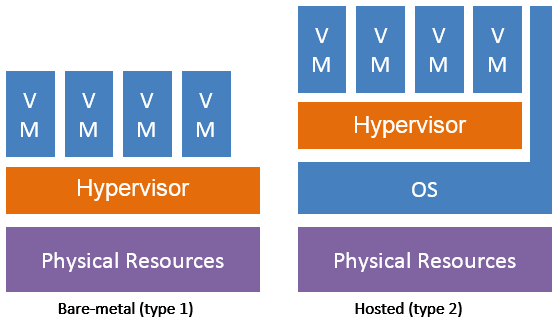
\includegraphics[width=0.5\textwidth]{virtualisation.png}
	\caption{The two types of virtualisation \protect\cite{virtualisation-security-guidance}}
	\label{fig:types-of-virtualisation}
	\vspace{3cm}
\end{figure}

When a business wants to buy a high performing computer for each employee, that would requires physical access to perform repairs, maintenance and management. Physical systems are more difficult to manage because they are distributed across a large area, making quick access slow or impossible. Another downside of not using virtualisation is non-scalable hardware utilisation. This is the case where one machine uses maximum resources but another one is idle. A computer that has predefined hardware specification cannot use more processing power than initially installed. 
Automating physical servers is also nearly impossible due to them lacking the necessary abstraction control layer.

These are some problems that virtualisation technology can solve. It is now a core part of most new desktop Intel© chips and is integral part of all server-grade processors as listed in the manufacturer's page \cite{intel-virtualisation-chip-support}.

This helps with performance, as a virtual machine can be configured on the fly to use flexible amount of resources or a shared pool of computational units. This technology also allows for easy server migration. A physical machine cannot be moved in a couple of minutes to a different continent (physical location) but a virtualised operating system can be "copy-pasted" at will for very little cost. Physical infrastructure is also prone to hardware-related bugs. This is a case when a software solution causes issues, because it was not tested on all the machines that run it. These physical machines might have different network cards, processors, lack certain hardware components or have older hardware version. The virtual platform has the benefit of abstracting away these components, ensuring that once tested, the software running on top of it would exhibit predictable behaviour \cite{nious-cloud-computing}[p.59].

How does virtualisation allow for easy \glspl{migration}? It achieves the task by abstracting away the available physical storage medium. On the virtualised host, they would appear as a large pool of \glspl{partition} with the data ready for management. Figure \ref{fig:vmware-datastore-image} shows a real world application, where more storage device can be added and the current one can be assigned/managed.

\begin{figure}[H]
	\vspace{1cm}
	\centering          
	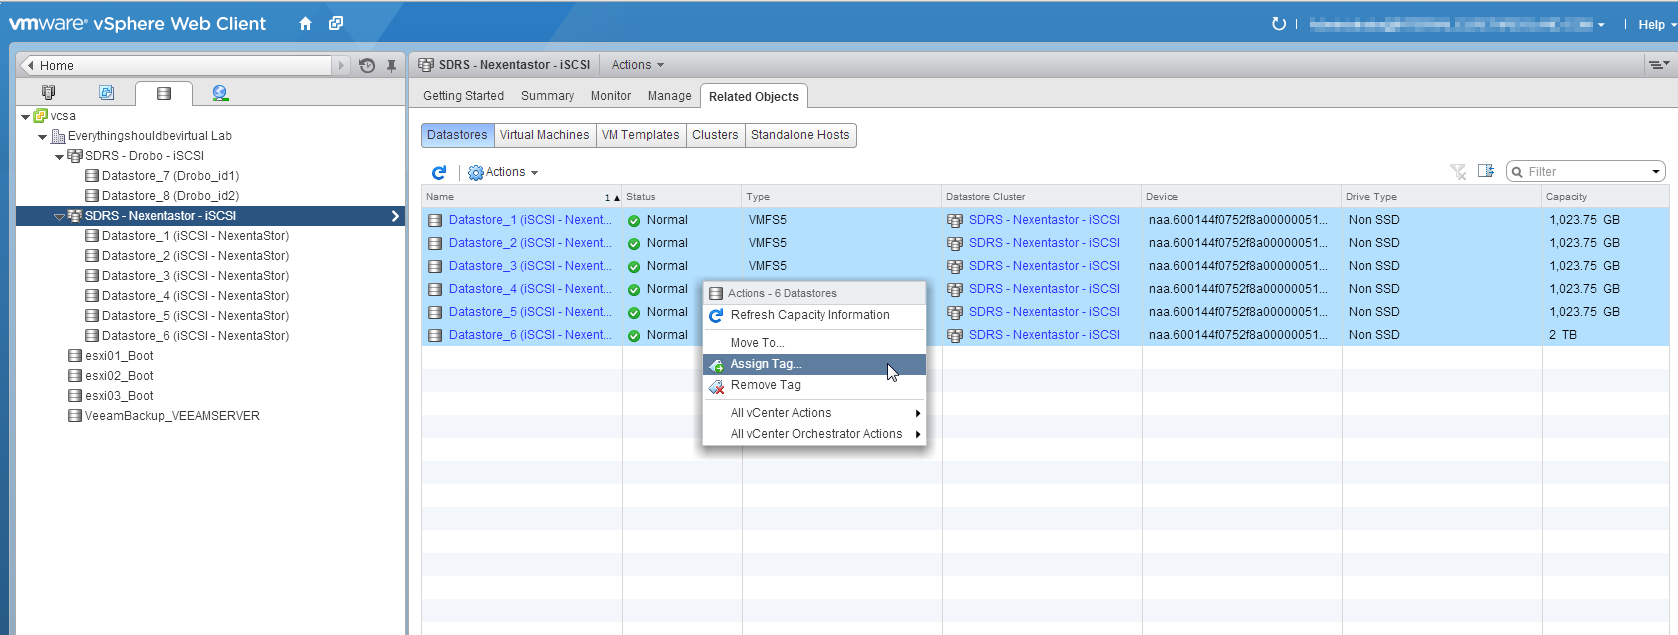
\includegraphics[width=1\textwidth]{datastore}
	\caption{VSphere data-store manager screen-shot. Source \protect\cite{vmware-storage-pool-screenshot}}
	\label{fig:vmware-datastore-image}
	\vspace{3cm}
\end{figure}

Having access to the virtualisation host allows the data of such system to be copied all at once to a different provider with the only requirement - have enough capacity to store the information. The alternative without using a virtualisation platform would be to gain physical access to each storage medium individually and copying the data incrementally.

\subsection{Purpose}
The project aims to utilise open-source virtualisation technology and make the process of managing and creating virtual machines automated through a web interface. The solution should allow a system manager to open a website, fill in a web form with enough information about the desired \gls{operating-system}, click a button and create it. After that, the person should be able to securely download identity file and connect to the machine.

The management website should also allow for the selection of predefined software packages. The solution should also show if the virtual machine is alive and allow the user to shut it down and bring it up. Port management should also be possible when building the machine. These features, alongside the benefits of virtualisation should create a secure infrastructure for many applications, from virtual office workstation, to server testing and deployment.

\subsection{Aim and Objectives}
\subsubsection{Aim}
Give developers a platform for easy deployment, management and monitoring of virtual servers.
\subsubsection{Objectives}

\begin{enumerate}
    \item Deploy a virtual machine of the user's choice through shell scripts
          \begin{enumerate}
              \item The main feature of the solution is the deployment of the virtual machine instances. The following will be achieved by using Oracle's virtualisation documentation for Virtualbox and the shell scripting language and the automation tool \gls{puppet}.
              \item The above will be achieved through the custom ruby module written for this dissertation - \texttt{deeploy}
          \end{enumerate}

    \item Configure firewall settings
          \begin{itemize}
              \item Will be achieved through the virtualisation technology's \gls{api}. The purpose is to add extra security layer to the guest \gls{operating-system}. Firewall settings are managed by a software called ufw - Uncomplicated Fire Wall
          \end{itemize}

    \item Allow console access and set up authentication credentials (SSH keys) for the instances
          \begin{itemize}
              \item The solution will generate unique shell credentials for each machine individually. Upon creation, the user should be able to download the credentials and use them to connect to the instance.
          \end{itemize}
    \item Monitor 'alive' status of the virtual instances
    \item Allow the user to install software from a predefined list
    \item Create a website that will manage and create the machines on the behalf of the user
\end{enumerate}

\newpage
\section{Background}
\subsection{Virtualisation and "The Cloud" }
"The most important feature of virtualisation that enables its cloud capabilities is the level of abstraction it provides. The key feature is the ability to hide the underlying hardware architecture." \cite{heterogenious-cloud-computing}[p.59]. The article Heterogeneous Cloud Computing: The way forward considers an architecture that interleaves different hardware components together, enabling their utilisation on-demand. For example, a cluster of graphic cards or processors that support different \gls{operating-system} architectures (x86, ARM, ATOM) can be attached in domain-specific tasks. Such set-up would allow the platform to be more flexible and less congested because these dedicated components would do the "heavy lifting. It also has the benefit of doing special computations - like rendering video much quicker and efficient. 

\begin{figure}[h!]
    \vspace{0.5cm}
    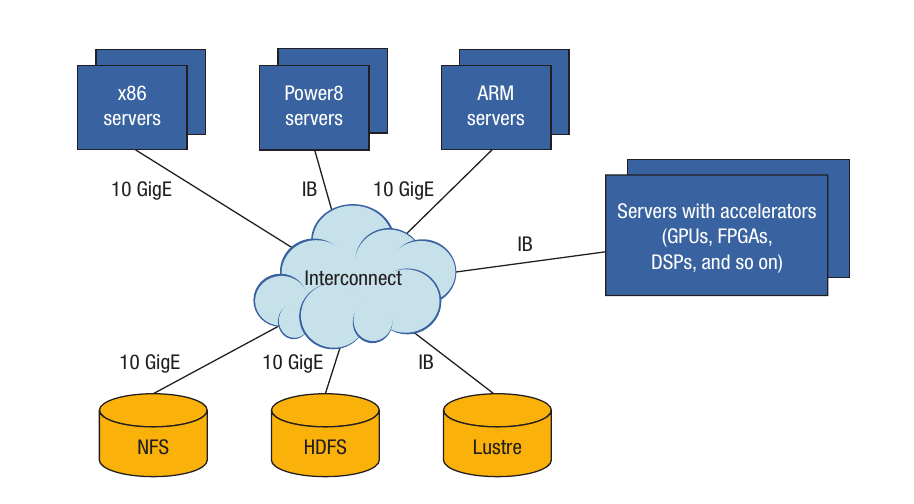
\includegraphics[width=12cm]{heterogenious}
    \vspace{0.5cm}
    \caption{Heterogeneous server configuration. Source \protect\cite{heterogenious-cloud-computing}[p.59]}
    \label{fig:birds}
\end{figure}

"Virtualization abstracts compute
resources—typically as virtual machines (VMs)—with
associated storage and networking connectivity. The
cloud determines how those virtualized resources are
allocated, delivered, and presented. Virtualization is not
necessary to create a cloud environment, but it enables
rapid scaling of resources in a way that nonvirtualized
environments find hard to achieve."\cite{intel-cloud-computing-guide}[p10]

Virtualisation provides the abstraction that makes it much easier to get data to and from the cloud. This technology is the basis for creating high availability services and applications when implemented properly.\cite{intel-cloud-computing-guide}[p10]. Intel's virtualisation and cloud computing guide talks about it as a way to provide corporate platform services in a more organised matter. The guide also covers making the infrastructure easier to organise from the standpoint of \gls{IT}. This is the case because these virtual servers are easier to diagnose and monitor as well as organise and automate \cite{intel-cloud-computing-guide}[p8].
Virtual machine diagnostics and monitoring is a practice where the behaviour of the machine is observed over a period of time. This includes network traffic, memory usage, \gls{cpu} performance and utilisation. It also contains information about how much disk storage the machine is taking and information about the machine's running status. Additionally, x86 computer architecture support hardware statistics counters. Performance counters are part of the kernel's sub-system and are the basis for providing reliable hardware information for monitoring and reporting \cite{rhel-performance-counters}.
This data can be used to gain insights into why a machine is malfunctioning. These counters can be vital in determining the type of issue with the machine (network related issue, hard-drive read-write failure, defecting processor, etc.). 
Network outages can be detected and accommodated for by analysing aggregated network statistics. This is useful in an event of denial of service attacks (DoS). High networking usage might indicate malicious behaviour such as artificial congestion - an attacker making numerious requests to slow down the service.
On the other hand, this type of monitoring can ensure on-demand scaling in critical moments. Legitimate customer demands must be met by allocating more hardware and network bandwidth as a result of increased demand.

Virtual machine organisation is the practice of managing a variety of components associated with the platform and its resources. The \gls{IT} department of an organisation is in charge of managing the physical storage on which the "virtual" platform is running. In the infrastructure disks are partitioned and organised in pools - then mounted over the network. This configuration uses S.A.N, or storage area network. This is a network entirely dedicated to transferring data between computer systems and the storage drives \cite{ibm-san-storage}[p.11].
Mapping physical drives to virtual ones over the network is a stepping stone in enabling any type of server infrastructure, including virtualised one, to have enough capacity to grow and meet the customer's demands. It also ensures the right level of redundancy, as a large portion of the hard drives can be put in place in case of a failure. Storing virtual machine on network drives makes it possible to copy machine instance from one cluster to another, or change data centres.

Any server infrastructure requires high bandwidth network connection, virtual networks are no exception. The network throughput of the platform depends on the internet service provider (ISP) physical connection speed. That network is used by the virtualisation platform and is converted to numerous private and public networks internally. The benefits of such abstraction is the ability to create flexible and disposable internal/external networks per machine or cluster of machines. The ability to share a network, or be in a private network is a security consideration. 		
This feature is important from the standpoint of security. For example, for a business logic application, one can set up a client-facing web server that is accessible from the global internet. The machine on which this application is running will have a database connection to another machine running a dedicated database software (mysql, postgresql, mongodb,etc.). The connection between the two machine would be configured as a private network. It ensures that nobody from the outside world has access to that database machine. This configuration is explored in Amazon's accessing database instance in a virtual cloud\cite{amazon-scenarios-for-accessing-db-instance-in-vpc}. The setup is shown in figure \ref{fig:amazon-scenarios-for-accessing-db-instance-in-vpc-figure}.

\begin{figure}[h!]
	\vspace{0.5cm}
	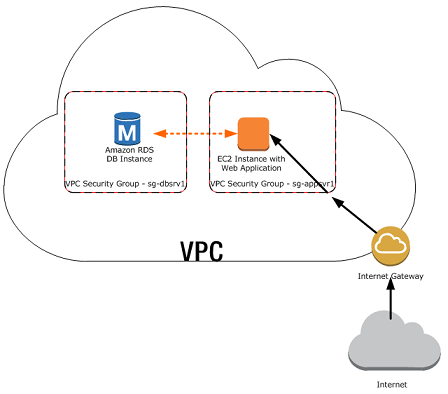
\includegraphics[width=12cm]{con-VPC-sec-grp}
	\vspace{0.5cm}
	\caption{Public facing gateway and internal network database. Source \protect\cite{amazon-scenarios-for-accessing-db-instance-in-vpc}}
	\label{fig:amazon-scenarios-for-accessing-db-instance-in-vpc-figure}
\end{figure}

It is impossible to talk about such infrastructure without considering the most important component of operations, the \gls{cpu}. When providing the hardware resources for computing, having enough calculation power is essential, otherwise each virtual machine would be slow and unresponsive. A server rack with many Intel\texttrademark \gls{xeon} or other server-grade chip are set to run on top of the virtualisation technology (\gls{virtualbox}, \gls{vmware} \ref{fig:types-of-virtualisation}. All of the computing resources are then also abstracted away. For example, when using \gls{vmware} \gls{vsphere}, instead of seeing every single processor, you are given the option of allocating certain amount of megahertz per instance. A guide on configuring \gls{cpu} usage is covered in VMware Cookbook \cite{vmware-cookbook}. CPU allocation screen is shown in figure \ref{fig:cpu-allocation}

\begin{figure}[h!]
	\vspace{0.5cm}
	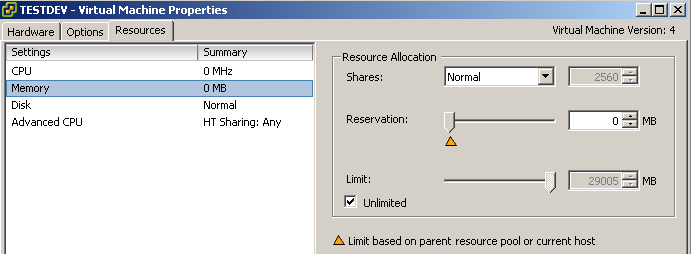
\includegraphics[width=12cm]{httpatomoreillycomsourceoreillyimages329633}
	\vspace{0.5cm}
	\caption{Resource and vCenter Management, allocating \gls{cpu} resources. Source \protect\cite{vmware-cookbook}}
	\label{fig:cpu-allocation}
\end{figure}

Considering the fact that all of these hardware components have to be managed by a human to ensure smooth operation during heavy and light loads, automation plays very big role in the process. Automation is the process of automatically creating \gls{virtual_machine} and dynamically allocating computing resources associated with it. Big cloud platforms such as \gls{amazon-web-services} and \gls{azure} have almost absolute automation. Azure even provide their tool as a service - Azure Automation \cite{azure-automation-overview}, Amazon use tools like \gls{chef} and in-house tools \cite{the-case-for-investing-cloud-automation}. Computing resources are allocated based on usage, where a paying customer can use a lot of resources for a certain price.

\subsection{Security}


\subsection{Similar in the field}
For the duration of my dissertation, I have evaluated a variety of technologies, frameworks and utilities that will allow me to achieve the goal of automated system deployment. The trial and evaluation of these technologies allowed me to find the most suitable and relevant methodology for moving forward. I also experimented with different "cloud" virtual machine deployment services to understand and evaluate the key requirements that ought to be provided by the platform.

Something that all major platform providers have in common is scalability and price model. The reason is that the platform allow for the hardware configuration parameters to be tuned at will within minutes. This means that when the \gls{virtual_machine} is created, later on the "hardware" resources can be modified and changed easily.

A commonality is the price model. All of the above mentioned platform providers use some form of pay-as-you-go. This means that companies requiring extra computation at time critical periods can take advantage of more computation. An example would be personal project of Harrison Kinsley for gene sequencing in his online learning series\cite{harrison-kinsley-tutorials}. He used 5 \glspl{gpu} for an hour to perform the necessary computation, then retrieved the results and then destroyed the machines. As a result, one can use sophisticated hardware for a fee with very little set-up overhead. 

\subsubsection{Amazon Web Services\texttrademark EC2}
\begin{center}
    \vspace{0.5cm}
    
\includegraphics[width=12cm]{2000px-AmazonWebservices_Logo.png}
    \vspace{0.5cm}
\end{center}

Amazon are the leaders in cloud deployment with 30\% world market share\cite{amazon-marketshare}. Their services range from providing \gls{dns} to deploying their custom virtual machines. Because of the widespread usage of their service and the fact that I have experience with working on their platform for professional or personal reasons, this is the main platform that inspired the work.

The main focus of the dissertation is not about the AWS platform, but about their service EC2 - virtual machine deployment.

EC2 allows a user to do the following:
\begin{itemize}
    \item
    Create scalable \gls{virtual_machine}. This includes selecting \gls{operating-system} type with a variety of options (Windows Server Ubuntu Linux, Red Hat Linux, Amazon Custom Images). They also offer machines for database only purposes (Amazon RDS).
    \item
    Select from a family of options that include general purpose machines, memory optimised, storage optimised, machines with dedicate \glspl{gpu} and storage optimised.
    \item 
    The amount of \glspl{cpu} to be used for the machine
    \item
    Amount of \gls{ram} in gigabytes to be used
    \item
    Storage capacity and storage type, e.g. how much and how fast it can be.
    \item
    Because they have their network load-balancers, it is also possible to configure the network performance of the machine.
    \item
    Configure IPV6 support. IPV6 is the updated internet protocol that allows for \begin{math} 3.4\times10^{38} \end{math}  network addresses to be allocated.
\end{itemize}

Some other benefits of EC2 is the ability to integrate with every other Amazon Web Service product. The service is also running on top of Amazon's network which ensures reliability and availability across many regions. 
EC2's pricing model has application for hobbyists and corporations alike due to the provided hardware options and the flexible pricing. Prices range from \$0.044 to \$14.400 per hour \cite{amazon-ec2-prices}. The service also receives publicity from having Netflix and Airbnb  hosted on their platform.
A downside to AWS is that they do not allow for custom \glspl{kernel} to be used and virtualised, leaving users to rely on the predefined images provided by the platform.

\subsubsection{Microsoft Azure}
Microsoft Azure is also among the biggest virtual machine and cloud computing providers in the world and has 10\% of the global market\cite{amazon-marketshare}.



\subsubsection{Heroku}

\newpage
\section{Planning}

\begin{center}
    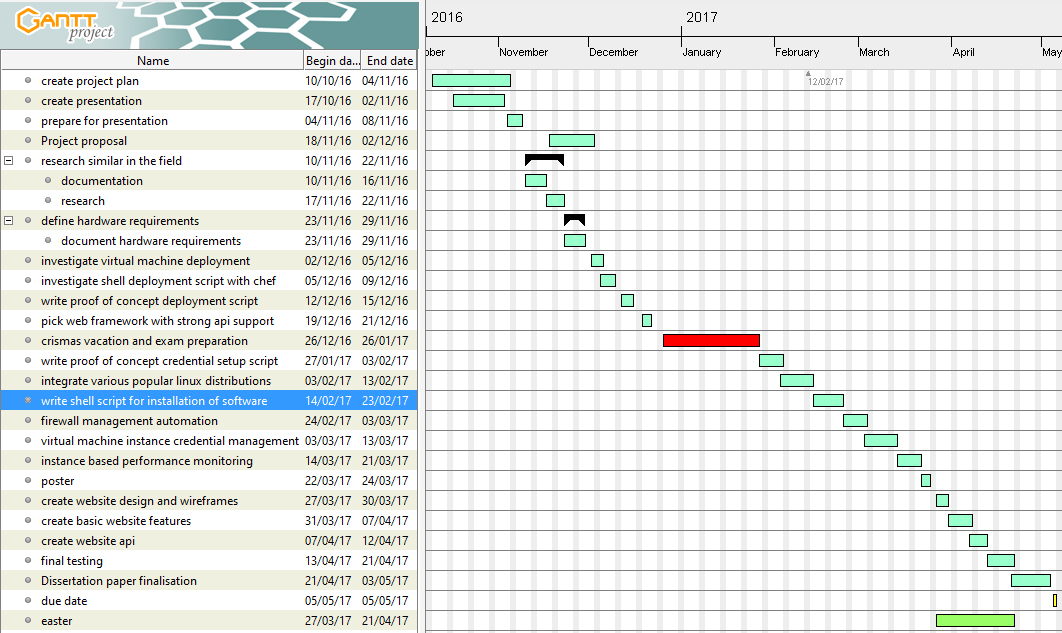
\includegraphics[width=12cm]{gantt.jpg}
\end{center}

As part of the development cycle, I have scheduled a meeting every fortnight with my supervisor to discuss work progress. During these meetings, I received feedback, raised concerns and showed progress in a \gls{standup} fashion. Occasionally, the meetings were not about progress update, but about demonstration of the work done so far with the purpose of obtaining feedback.

\subsection{First Semester}
When creating the project plan, two core stages were taken into consideration. The first stage is semester one. During that period, the ground work was laid, on which all future development and testing work was based. This is a critical moment into the building process. It allowed for a more in-depth research using materials created by the leading experts in the field (Amazon, Intel, Oracle). These documents helped gaining more understanding in various aspects of building cloud-ready applications, infrastructure security and automation.

The research helped when rationing about the features that need implementing. It also illustrated the scope, and the challenges that need to be faced. The research gave an insight into why this problem requires solving, and pointed me to open-source projects that achieve parts of the work.

The first semester was not only about research, but also about describing the constrains, limitations and infrastructure decisions that need to be made in order to demonstrate a  product that has real-world applications.
The materials helped me also to identify potential risks and issues that might arise, such as the security risk of running multiple virtual machines onto the same physical space. This is a potential risk situation, as an attacker can read the private data of another machine if the person gets access to the memory of the "host".

Work also went into creating presentation and project proposal for the upcoming work, which give an outline and highlighted the features that the work addresses.
When creating the presentation, I wanted to be as generic as possible as not to present information and ideas that the additional research might prove impossible to implement or not practical.

\subsection{Second Semester}

The tasks accomplished during the second semester are related to implementing, refining, iterating, evaluating and documenting the solution. This is the time where all the main features, functional and non-functional requirements got developed, tested and documented. It must be noted that for the most part, each cycle was not incrementally tackled, but instead, numerous development-testing-documenting phases were used to achieve the final result.
\begin{center}
    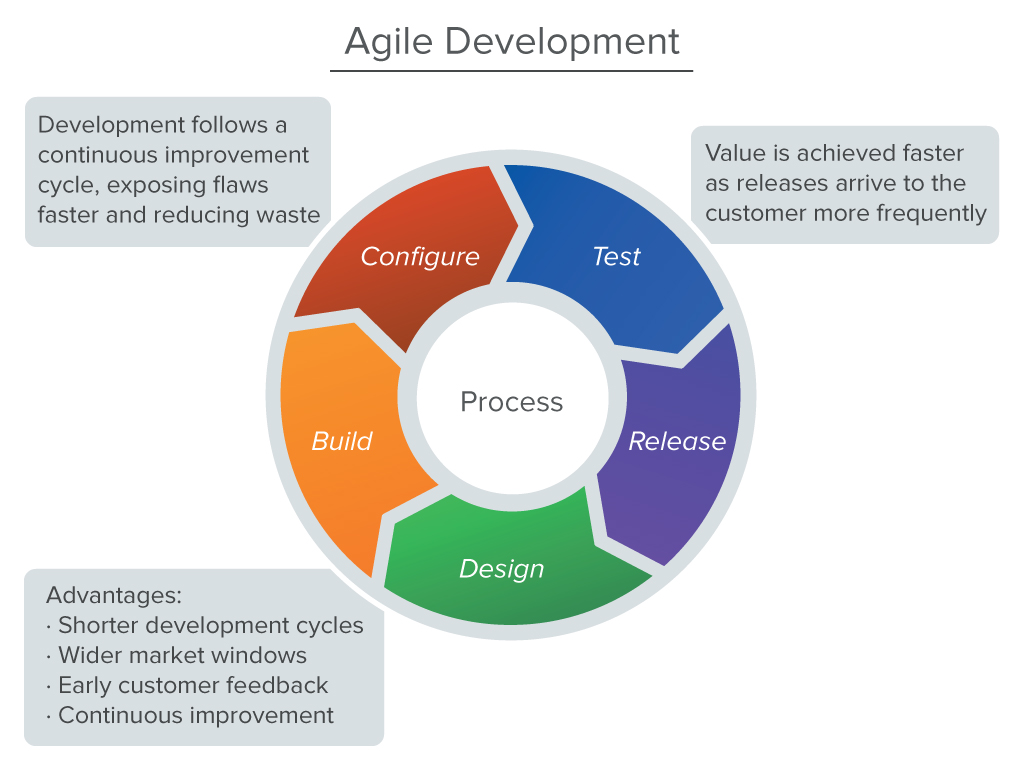
\includegraphics[width=12cm]{agile.jpg}
\end{center}

For the most part, the project was completed using the agile methodology. Each cycle that shaped the final product is described below.
\subsubsection{Developmen}
As planned, I broke down the main objectives into subtasks and tackled them one-by-one. My initial plan is not to develop the whole system and assemble the parts together at the end, but to build a minimum viable product (MVP) and increment onwards.

This was done in order to assure that the platform can be built with the available tools and that the requirements can be met at the end of the project.

Being able to create a virtual machine with a known \gls{ipaddress} from a script was the first thing that had to be accomplished. Creating custom users, opening ports and creating the web interface was planned later as something that could be built on top of the "core" product.

\subsubsection{Learning period}
For the duration of this project, a variety of new technologies were tried and evaluated, such as \gls{vagrant}, \gls{puppet}, \gls{ruby-on-rails}, \gls{ruby}.

As part of the learning cycle, the official ruby programming language manual was used. It helped gain proficiency to understand the fundamental constructs that were used throughout the tutorials, articles, blogs and other learning materials. The process taught me about declaring variables, scopes, for loops and any extra syntax unlike other programming languages. To get up and running with \gls{ruby}, the period between first and second semester was planned to build basic command line programs.

Another part of the development strategy was to do a small web project using ruby on rails just to get a feeling of what is possible in terms of rapid development and ease of use. This small project included building forms, validation, manipulating database objects and creating \gls{html} pages. This was done in February (the beginning of second semester), with the purpose of determining if this tool is right for the job

The task of learning \gls{puppet} was achieved by creating end-to-end automation scrip of the current set-up of my desktop machine. Puppet's power is to get a machine's configuration to a known state and ensure all software packages are present. Doing this exercise was overall a good practice, as it led to a faster implementation and integration later on when working on the actual platform.

\subsubsection{Documentation}
The initial plan as stated in the project proposal is to document the work during each stage of the process, like implementing a new feature. I later decided to not strictly follow that plan, as there were many components that changed drastically. For example, in the beginning, I planned to use chef for configuration automation and management. After evaluating and experimenting with it for 5 days, it was apparent that the set-up overhead was slowing down the actual development process. 

Because of that experience, the dissertation write-up process was changed to documenting features only when they are established.


\newpage
\section{Methodology}
\subsection{Overview}
This chapter aims to give a more in-depth view into the process of scoping, developing, planning and building the application. This ranges from picking the tools to limiting the scope, making assumptions, as well as the scheduling of each task. Creating such a platform from nothing is a daunting task even for an experienced senior software engineer.

For the above reason, the initial research into building the right tool-chain was essential to the success of the project.

The development methodology can be broken into the following steps:
\begin{enumerate}
    \item
          Research into virtualisation technology to understand the underlying architecture.

    \item
          Select free and open-source software components that can be coupled together to orchestrate and utilise above mentioned technology. The public libraries used also allowed me to extend, modify and build on top of during the development process.

    \item
          Build a set of core and advanced features. Core features are essential for a good operational and usable solution. Advanced features are the things that make this solution go above and beyond the scope of existing applications.

    \item
          Integrate components into one final solution

    \item
          Do sufficient testing to ensure that the platform behaves as expected.
\end{enumerate}

\subsection{Constrains}
Because of the limited duration of the dissertation and the immense work that has to be carried throughout the implementation (testing, documentation, development, debugging, planning, etc.) certain constrains had to be put in place to ensure that the project will be completed within the appropriate period.

The initial constrain that I have defined is limiting the solution to a single host. This work is done as a proof-of-concept system that has the potential of being scaled up and extended to support "real-world" application.
Creating a distributed and scalable implementation of this work goes beyond the scope. This is not to say that it is limited to single host, but testing and planning guarantee that it will be fully functional under such condition.

As a future task, it would be possible to deploy multiple instances of the underlying infrastructure that are managed and synchronised with a technology like puppet or chef. Then, creating virtual machines can be done via a manager machine that picks a host based on a round-robin algorithm or based on load. Additional implementation steps must be carried out to ensure that the web platform and the manager understands the physical location of the virtual machine. Physical location references to the real hardware (the host) running the virtual machine.

Another assumption and a constrain is the availability of a network interface. To simplify the development process and allow me to isolate different environments. A network environment is the space in which all the virtual machines have visibility of one another. It also makes it possible to allocate different network addresses dynamically and verify availability of resources. Another important bit is the fact that one must be connected to the network environment to communicate with the machines inside of it. I have taken advantage of VirtualBox's host-only networking interfaces, and have created multiple instances that allow me to create machines independent of each other when developing and testing.

When further extending the solution, additional work has to be carried out to ensure integration with a public \gls{dns} server, and some adjustments ought to be made to allow the production \gls{dns} to allocate \textcolor{red}{DHCP} ip addresses to the virtual machines.

The solution aims to orchestrate and automate generic virtual machine deployment, but creating a solution that enables every \gls{operating-system} to be deployable would require extensive amount of extra work. Future work can make it possible to deploy Windows, Mac OS and more Linux variants as part of the infrastructure, but this is yet not the case.

Windows is not supported yet, as it has completely different architecture and has a separate interface for managing networking, users, installation and permissions. Doing windows deployment also requires licensing of their \gls{operating-system}. Another constrain in working with windows is that not many core components are configurable or accessible via a script making automation very difficult or impossible.

Mac OSX virtual deployment was also something left for future. It also has similar issues to windows virtualisation (licensing, exposed \gls{api}).

Finally, as it comes to Linux virtual machine deployment, I have opted to cover

For the purpose of this work, I have decided to limit the scope of allowed Linux distributions to Ubuntu, Centos and debian, but it is important to note that the architecture allows extending that list.

\section{Work}

A hypervisor is a computer software or hardware that creates the platform layer to a virtual machine and makes it possible to host multiple instances with different configurations \cite{ibmvirtualisation}.

Initially, the plan was to use a hypervisor virtualisation solution such as \gls{virtualbox} and \gls{vmware} just by themselves, and use the \gls{bash} shell scripting language to interface directly with them. A decision was made to use Virtualbox, as it is an \gls{open-source} software solution, has strong community, allows third party plug-ins and is a solution build by Oracle - a large software corporation. There are other alternatives (gnome boxes, CHROOT), but what influenced the choice is that virtualbox is configurable and can be controlled from the command-line straight out of the box. Another deciding factor was also the extensibility that it offers with third party modules developed by the community and the core team (guest additions, virtualbox standard development kit).

Another reason for not choosing a more unpopular technology is due to the willingness of an adopter to switch their entire virtual infrastructure to it. The Virtualbox software is very popular \cite{_NEEDED_}, and as such, it would make the transition to the platform easier.

During the period when researching Virtualbox, the command-line \gls{api} documentation was used extensively. In the process, a variety of customisable parameters when building a virtual machine were discovered, like the different possibilities in setting up networks (private, network shared, host only, etc.), exposing ports, as well as different hardware configurations (RAM, hard drive, CPU count). After using the command line tools and writing a simple shell scripts for managing creation of different resources, a decision was made to use a tool that manages the different technical details of each virtual machine. Instead of building the manager from scratch, an open-source hypervisor provisioner software was used instead. The tools is called \gls{vagrant}.

\subsection{Vagrant}
Vagrant by Hashicorp, is a tool built by a company specialising in easy virtual machine configuration management and set-up Their \gls{api} provides the following features.

\begin{itemize}
	\item
	Allow the administrator to create a \gls{vagrant} configuration file (called Vagrantfile), which describes end-to-end each operation that will be performed to the virtual machine instance (including the Linux distribution that will get installed on it).
	\item
	Create a system compatible with their platform starting from a bare configuration and incrementally building a bespoke instance. These instances can be managed and shared on the internet.
	\item
	Managing network interfaces
	\item
	Configure ports
	\item
	Allow port access to adapter network (in private networks)
	\item
	Create a custom machine compatable with the platform
	\item 
	Kick-start automation by running one of the supported automation frameworks (chef, puppet)
\end{itemize}

\subsection{Workflow}
The framework that was created uses a \gls{virtual_machine} instance object and authenticated user that owns it. When the user fills the web form with the relevant information, it will pass the configuration values directly to a virtual machine class. This class contains a dynamic configuration, which ensures that the solution is distribution agnostic. Here, the term distribution references to the different versions of Linux (Ubuntu, fedora, Centos, arch Linux). Separating dependency specific configuration by sub-classing a configuration object allows for a quick way for the project to be extended to accommodate for new distributions.

To do so, folder with the name of the new distribution must be placed in lib/configurations that describes the configuration specific settings that include updating and installing common software packages.

The framework also uses UNIX environmental variable to manage infrastructure state. For the  purpose of developing and testing, I have created two main isolated environments - testing and development.
The most notable usage of such environment is the virtual host-only network that ensures that the virtual interfaces do not clash during testing and development. The two interfaces are \texttt{vboxnet0} and \texttt{vboxnet1}. One is for general purpose development, the another is for testing. A special host-only adapter is used to have an isolated ip range that is network agnostic, for example, on a \gls{natnetwork}, some IP addresses might be reserved or used, this case will cause a clash and the virtual machine will not be reachable.

\subsection{Architecture}
When considering the architecture of the system, a list of factors were evaluated when building the solution. One is having few well consolidated moving parts, ensuring flexibility and extensibility. For that purpose the programming language \gls{ruby} was chosen. It is a suitable for system automation as it is very expressive and is for the most part platform independent (interpreted). Its suitability comes also from the available tools \gls{vagrant} and \gls{puppet} which allow end-to end integration when developing and testing. The \gls{ruby} programming language also draws inspiration from the Perl programming language. One of the Perl's strengths is its ability to be a more powerful shell scripting language as well as a general purpose language. This is the case as it has quick syntax for executing shell scripts directly and get STDOUT, STDERR and exit-codes quickly. It does also has native implementation of common UNIX tools, like grep, wget and awk (core GNU utilities).\cite{perl-programming-language-shell-scripting}

Because the Ruby language draws inspiration and shares similar features with Perl, it makes it a great modern and powerful language to use in this domain-specific problem. The language benefits from it bein written in 1995, and being very mature. For that reason, there is a great amount of online help and third party library of great quality.

\subsection{The deeploy module}

\begin{figure}[h!]
	\vspace{0.5cm}
	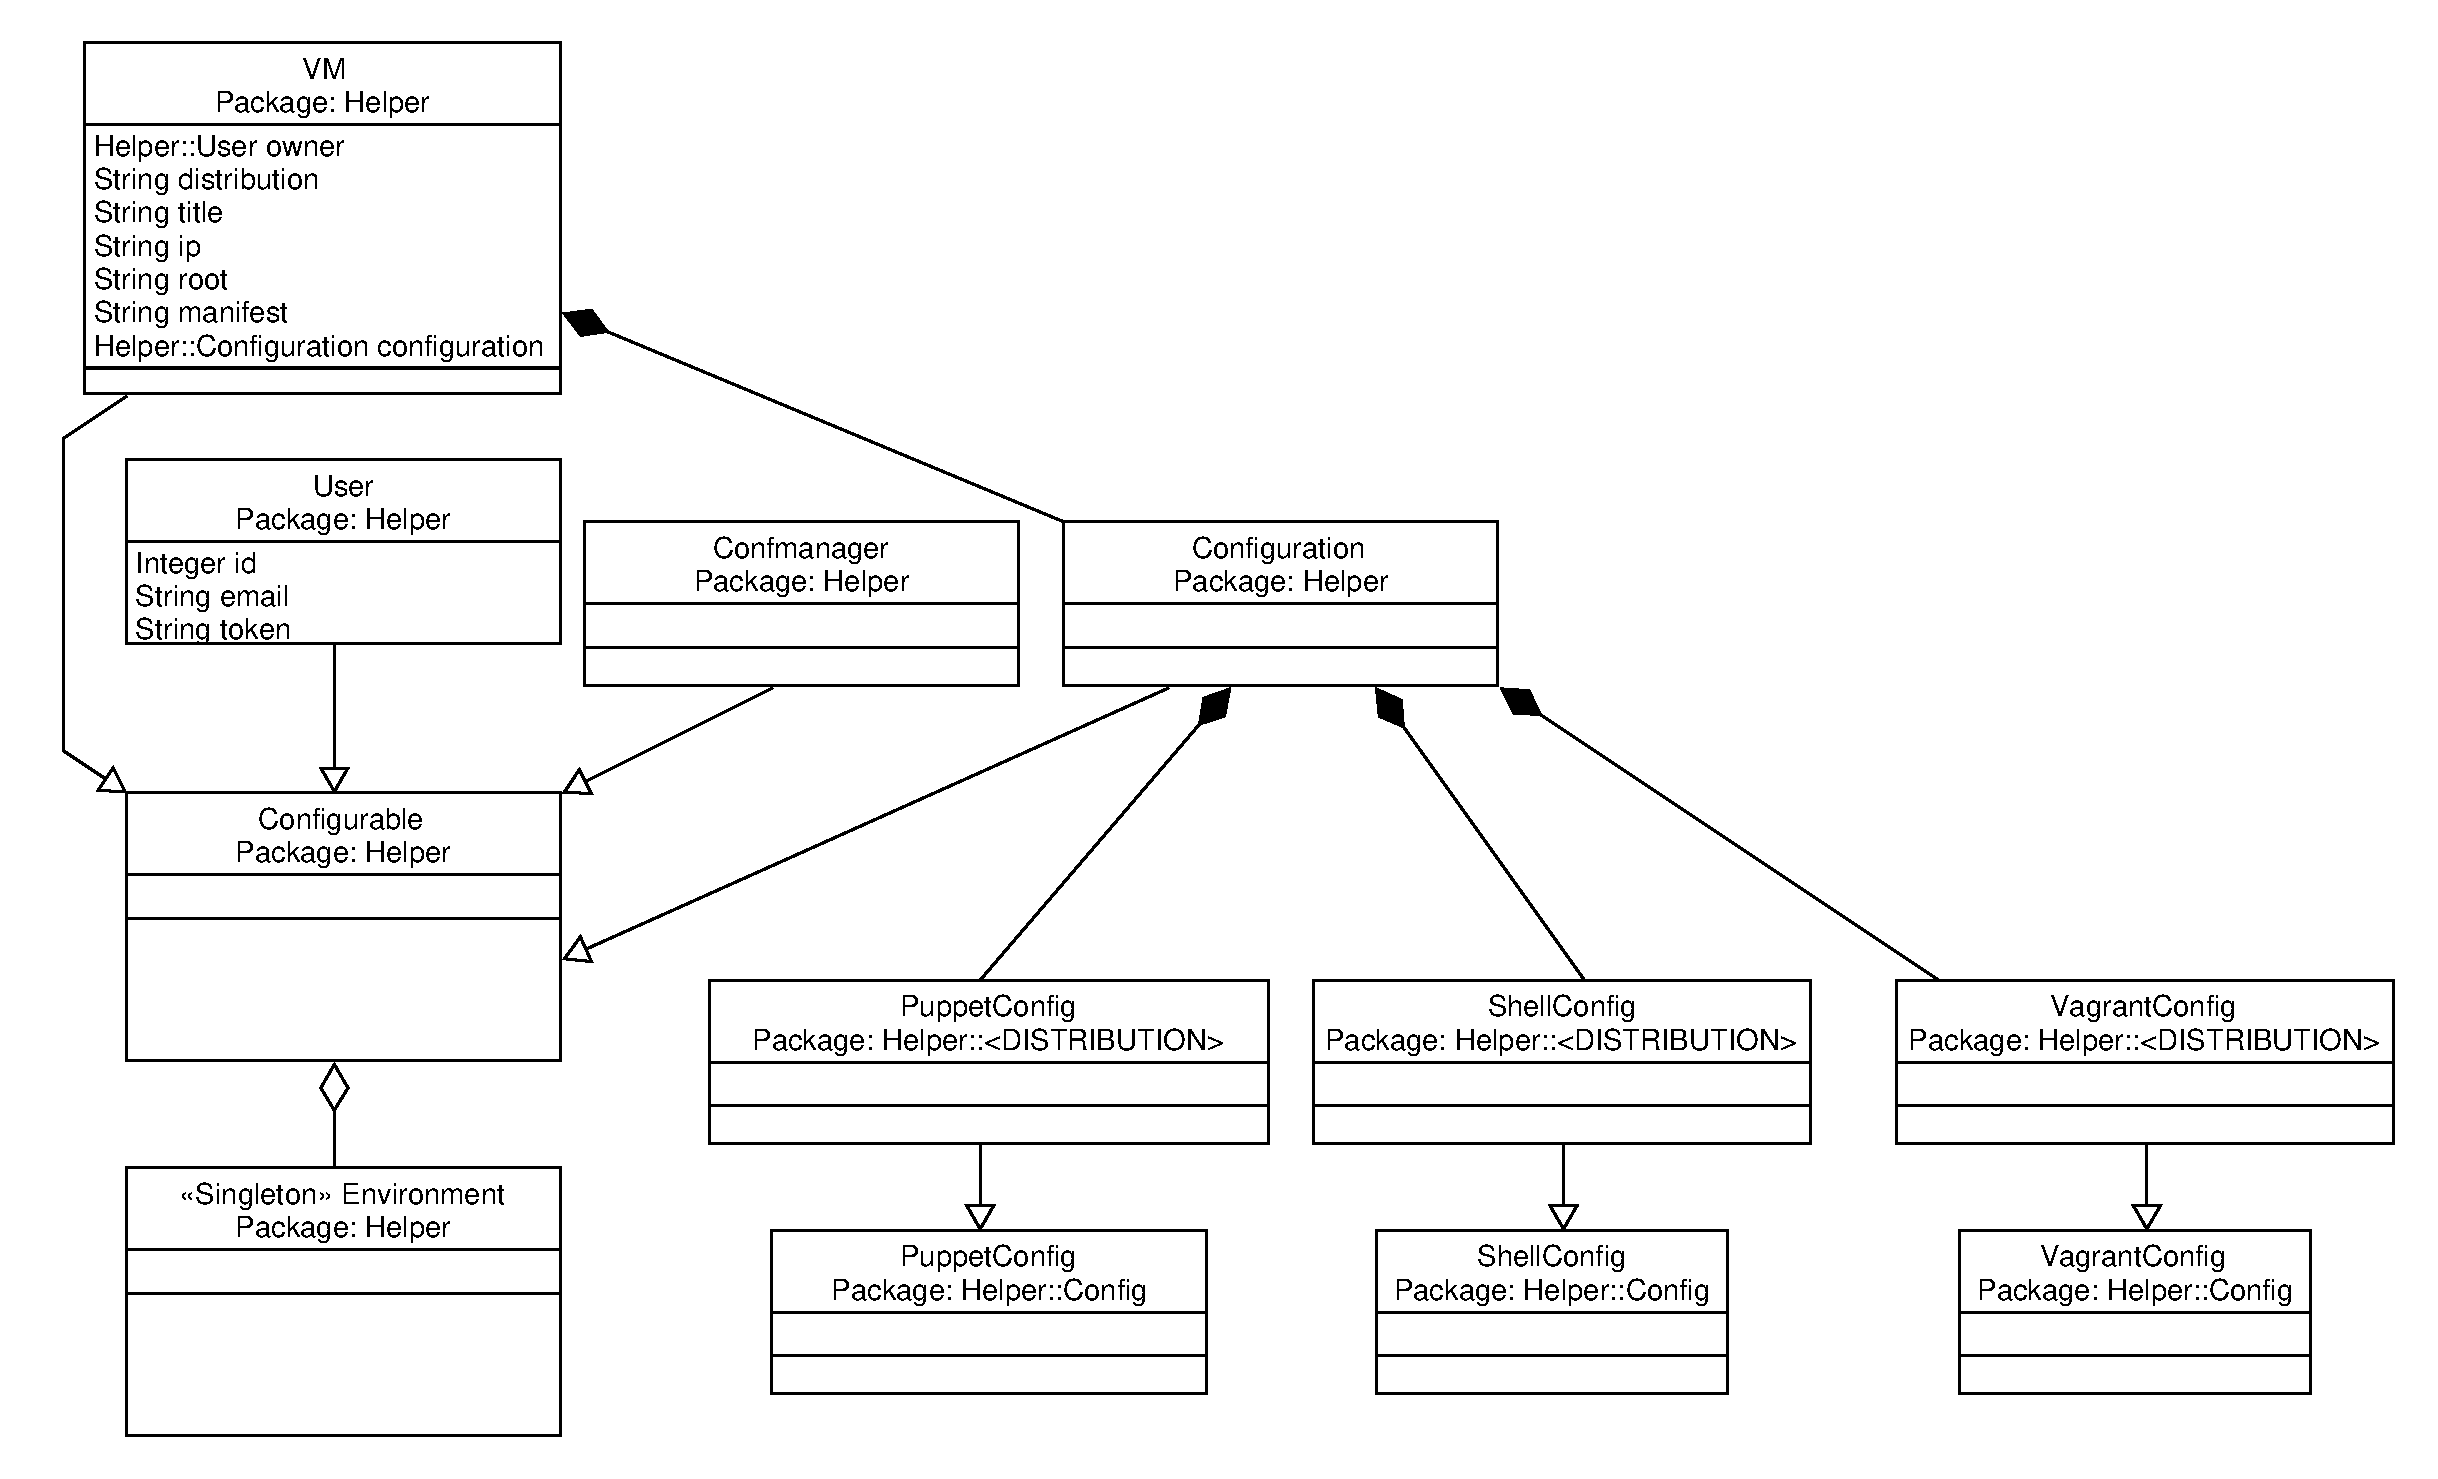
\includegraphics[width=12cm]{architecture}
	\vspace{0.5cm}
	\caption{Architecture of the deeploy module}
	\label{fig:deeploy-architecture}
\end{figure}

The first component of the work is a ruby module designed specially to act as a back-end for the entire solution. A module is a collection of programming functions and libraries that are bundled together to achieve a particular task. In \gls{ruby}, modules are called gems. For writing my first \gls{gem}, the official ruby guide was used as guide \cite{ruby-official-guide}. 

The file \texttt{lib/deeploy.rb} is what sets up the database connection and bootstraps the whole module by auto-loading every component. To ease integration, the file loads configuration properties from the file \texttt{lib/config/application.yml}. \texttt{Application.yml} contains configuration for production, development and testing, this is to allow separation and configuration of different parameters. The file specifies location of the database file when in development, or it has the database drivers in production with information about connection parameters. The file also describes the network interfaces to be used in each environment.

\texttt{lib/deeploy.rb} has a helper method that returns the current network interface and \gls{netmask}, this function is responsible for generating \glspl{ipaddress} and also for verifying that the virtual network is up and running. It does so by issuing commands for bringing up the virtual networks \texttt{vboxnet} up, then using network sockets to extract relevant information. This function is the programatic equivalent to the command \texttt{ifconfig or ipconfig}.

The file also contains a static function that returns a map of all supported distributions and the associated \gls{vagrant} machine. The function is helpful when validating creation, and will error out if the \gls{distribution} name is not in the list. When extending the supported distribution, this function needs updating. 

Similarly to the supported \glspl{distribution} function, there is a static function to return the supported packages list, used for displaying the options and validating unsupported packages.

The module provides a function slugify, its purpose is to convert string with special characters and spaces to a set of words and dashes, non-ASCII characters are stripped.

\gls{ipaddress} helper function checks if the supplied  is part of the current network by using ruby's \texttt{ipaddr} build in module. 

The file \texttt{lib/vm.rb} contains the code for managing the virtual machine instances, the class is called \texttt{Deeploy::Configurable::VM}. The class inherits from \texttt{Configurable}. Calling \texttt{VM.new} contains validators that raise errors upon initialising the class inappropriately. 
The method is responsible for specifying the distribution, available resources, configuration destination, name of the instance, packages, open ports and prepares it for creation. A design decision was made to allow a machine to be configured with the \texttt{new} operator and then created by issuing \texttt{machine\_instance.build()}.

The method \texttt{VM.alive()} verifies if the machine is alive by trying to listen on \gls{ssh} port, if it fails within a time-out, the machine is updated to state of not alive.	

\texttt{VM.get()} is used when performing power up, power down and destroy virtual machines. It queries the database and discovers everything about the instance, from packages, to \gls{ram} and location of configuration files.

The virtual machine is built only when an instance is initialised properly by calling \texttt{VM.new} with the correct arguments and then invoke \texttt{VM.build()}. The design decision to have a separate functionality of bootstrapping instances was mainly for cleaner testing by compartmentalising the components into smaller elements. The \texttt{build} method also accepts a boolean argument. This argument tells the current build if it is in "dry-run" mode. The mode, the machine will create directories and configuration without actually bringing the instance up and running. This is again, done for testing reasons - they verify that different \glspl{distribution} have appropriate configurations.

During the invocation of the \texttt{build} method, a \gls{bash} shell is forked and it executes the \gls{vagrant} command that brings it on-line and installs all dependencies. The shell command also tells the script to write all output to a text file in the machine directory, the file is called \texttt{vagrant.log}. Because the process takes a long time to finish, an axillary function \texttt{\_wait\_on\_build} is used. This function constantly goes through the contents of the log file and checks what is the current building state of the instance. Typical states are building the base, installing puppet, setting up dependencies, installing packages and the state everything has finished.

Additionally, the process of creating a virtual instance is using a custom image that has a variety of pre-installed software and firewall rules specially created for the dissertation. The purpose is to increase deployment time and allow for a more controlled package list.

The process of building a virtual machine by the \texttt{deeploy} module is also illustrated in figure \ref{fig:deeploy-build-flow}

\begin{figure}[h!]
	\vspace{0.5cm}
	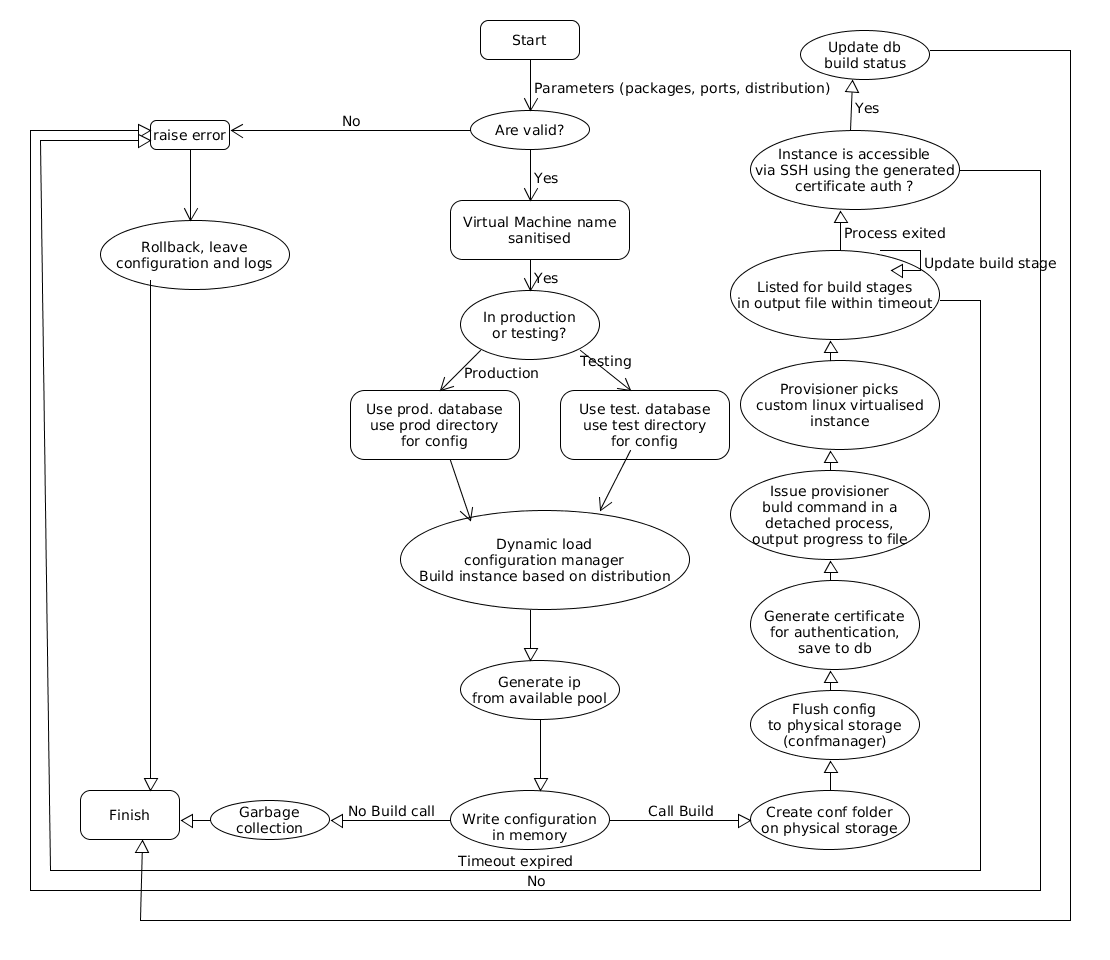
\includegraphics[width=12cm]{build-flow}
	\vspace{0.5cm}
	\caption{Deeploy build flow}
	\label{fig:deeploy-build-flow}
\end{figure}


\subsection{Issues}
TALK ABOUT CHDIR ISSUE THREAD SAFE AND ABOUT HEALTH MONITORING DEAMON INSTEAD OF CHECKING EVERYTIME DUE TO THE SLOWDOWN

\newpage
\section{Evaluation and Testing}
http://guides.rubygems.org/make-your-own-gem
\newpage
\section{Conclusion}

\newpage
\section{References}
\bibliography{research}

\renewcommand{\bibname}{}

\newpage
\section{Glossary}
\printglossary
\newpage
\section{Appendix}


\begin{filecontents*}{research.bib}
    
    @online{amazon-marketshare,
        author = {Synergy Research Group},
        title = {Amazon Leads; Microsoft, IBM \& Google Chase; Others Trail},
        url = {https://www.srgresearch.com/articles/amazon-leads-microsoft-ibm-google-chase-others-trail},
        urldate = {01.08.2016},
        note = {Accessed: April 02, 2017}
    }

    @online{harrison-kinsley-tutorials,
        url = {https://www.youtube.com/user/sentdex/about},
        note = {Accessed: April 03, 2017},
        title = {Python Programming tutorials},
        author = {Harrison Kinsley}
    }
    
    @online{a,
        author = {Internet Live Stats},
        title = {Google Search Statistics},
        url = {http://www.internetlivestats.com/google-search-statistics},
        urldate = {03.05.2014},
        note = {Accessed: November 26, 2016}
    },

    @online{b,
        author = {Techopedia Inc},
        title = {Definition of Virtualization},
        url = {https://www.techopedia.com/definition/719/virtualization},
        urldate = {2014},
        note = {Accessed: November 26, 2016}
    },

    @online{vagrant-definition,
        author = {Hashicorp},
        title = {WHY VAGRANT?},
        url = {https://www.vagrantup.com/docs/why-vagrant/},
        note = {Accessed: 27.03.2017}
    },

    @online{puppet-definition,
        author = {Puppet Labs},
        title = {Puppet Documentation},
        url = {https://docs.puppet.com/},
        note = {Accessed: 27.03.2017}
    },

    @online{ruby-on-rails-definition,
        author = {Ruby On Rails team},
        title = {Getting Started with Rails},
        url = {http://guides.rubyonrails.org/getting_started.html},
        note = {Accessed: 27.03.2017}
    },

    @online{ruby-definition,
        author = {Ruby team},
        title = {Ruby homepage},
        url = {https://www.ruby-lang.org/en/},
    note = {Accessed: 27.03.2017}
    },


    @online{ictonline,
        author = {ITU ICT},
        title = {ICT Facts and Figures 2016},
        url = {http://www.itu.int/en/ITU-D/Statistics/Documents/facts/ICTFactsFigures2016.pdf},
        note = {Accessed: March 08, 2017},
        year = {2015}

    },

    @book{what-is-migration,
        author    = {Birgit Kreuz, Antony Higginson},
        title     = {Migrating Oracle Databases},
        year      = {June 2014},
        publisher = {Oracle Corporation},
    }


    @book{what_is_partition,
        author    = {Bill Calkins},
        title     = {Oracle Solaris 11},
        year      = {2013},
        publisher = {Prentice Hall},
        isbn      =  {978-0-13-300710-7},
    }

    @online{what_is_virtual_machine,
        author    = {Oracle corporation},
        title     = {Oracle\texttrademark VM User's Guide},
        year      = {2015},
        url = {https://docs.oracle.com/cd/E20065_01/doc.30/e18549/oraclevm.htm#CACFJCFH},
        note = {Accessed: March 08, 2017},
    }

    @book{SecuringtheCloud,
        author    = {Vic (J.R.) Winkler},
        title     = {Securing the Cloud},
        year      = {2011},
        publisher = {Elsevier/Syngress},
    }

    @book{ibmvirtualisation,
        author    = {Shannon Meier},
        title     = {IBM Systems Virtualization: Servers, Storage, and Software},
        year      = {April 2008},
        publisher = {IBM},
    }

    @book{whatisnat,
        author    = {Javvin Technologies Inc},
        title     = {Network Protocols Handbook},
        year      = {2005},
        publisher = {Javvin Technologies},
    }

    @online{intel-cloud-computing-guide,
        author = {Intel Corporation},
        title = {Virtualization and Cloud Computing},
        year = {2013},
        url = {http://www.intel.com/content/dam/www/public/us/en/documents/guides/cloud-computing-virtualization-building-private-iaas-guide.pdf},
        note = {Accessed: April 04, 2017},
        
    }

    @online{amazon-ec2-prices,
        url = {http://www.ec2instances.info/},
        title = {Amazon EC2 Instance Comparison},
        author = {Garret Heaton},
        note = {Accessed: April 04, 2017},
    }

    
    @online{techopedia-it-definition,
        url = {http://searchdatacenter.techtarget.com/definition/IT},
        author = {Margaret Rouse},
        title = {Information Technology (IT) }
        year = {April, 2015},
        note = {Accessed: April 05, 2017},
    }

    @online{rhel-performance-counters,
        url = {https://access.redhat.com/documentation/en-US/Red_Hat_Enterprise_Linux/6/html/Developer_Guide/perf.html},
        title = {Performance Counters for Linux (PCL) Tools and perf},
        author = {Red Hat, Inc.},
        note = {Accessed: April 05, 2017},
    }

    @book{ibm-san-storage,
        author    = {Jon Tate},
        title     = {Introduction to Storage Area Networks},
        year      = {2016},
        publisher = {IBM},
        isbn      =  {073844233X},
    }

    @book{heterogenious-cloud-computing,
        author    = {San Murugesan},
        title     = {Heterogeneous Cloud Computing: The Way Forward},
        year      = {2015},
        publisher = {BRITE Proffesional Services},
        isbn      =  {073844233X},
        url = {hhttp://www.isi.edu/sites/default/files/users/jwalters/papers/computer_2015.pdf}
    }

    @book{vsphere-definition,
        title = {VMware vSphere Introduction},
        author = {VMware, Inc.},
        year = {2009}
    }

    @online{vmware-definition,
        url = {http://www.nytimes.com/2009/08/31/technology/business-computing/31virtual.html},
        note = {Accessed: April 10, 2017},
        author = {STEVE LOHR},
        year = {August 30, 2009}
        title = {Challenging Microsoft With a New Technology}
    }

    @misc{heterogeneous-network-table,
        url = {http://www.isi.edu/sites/default/files/users/jwalters/papers/computer_2015.pdf},
        title = {}
    }

    @online{perl-programming-language-shell-scripting,
        url = {http://blogs.perl.org/users/buddy_burden/2012/04/perl-vs-shell-scripts.html},
        title = {Perl vs Shell Scripts},
        author = {Buddy Burden},
        year = {April 16, 2012},
        note = {Accessed: April 10, 2017},
    }

	@online{virtualisation-security-guidance,
	    url = {https://www.ncsc.gov.uk/guidance/virtualisation-security-guidance},
		title = {Virtualisation Security Guidance},
		author = {National Technical Authority for Information Assurance},
		year = {May 19, 2016},
		note = {Accessed: April 10, 2017},
	}

	@online{intel-virtualisation-chip-support,
		url = {http://www.intel.com/content/www/us/en/support/boards-and-kits/desktop-boards/000005758.html},
		title = { Intel® Virtualization Technology Requirements},
		author = {Intel Support},
		year = {Feb 28, 2017},
		note = {Accessed: April 10, 2017},
	}

	@online{vmware-storage-pool-screenshot,
		author  = {Lee Smith Jr.},
		title   = {vSphere 5.5 Storage Profiles Are Now Storage Policies},
		year    = {October 28, 2013},
		url     = {http://everythingshouldbevirtual.com/wp-content/uploads/2013/10/16-48-29.png},
		note = {Accessed: April 15, 2017},
	}

	@online{amazon-scenarios-for-accessing-db-instance-in-vpc,
		author = {Amazon Web Services},
		title = {Scenarios for Accessing a DB Instance in a VPC},
		year = {September 27, 2015},
		url = {http://docs.aws.amazon.com/AmazonRDS/latest/UserGuide/USER_VPC.Scenarios.html},
		note = {Accessed: April 20, 2017}
	}

	@book{vmware-cookbook,
		title = {VMware cookbook},
		author = {Ryan Troy},
		year = {2012},
		publisher = {Oreilly Media}
	}

	@online{azure-automation-overview,
		author = {Matt Goedtel et .al},
		year = {October 5, 2010},
		title = {Azure Automation overview},
		note = {Accessed: April 20, 2017}
	}

	@online{the-case-for-investing-cloud-automation,
		author = {The Case for Investing in Cloud Automation},
		author = {Kate Miller},
		year = {October 7, 2016},
		title = {The Case for Investing in Cloud Automation}
	}

    @online{ruby-official-guide,
		author = {RubyGem Team},
		title = {Make your own gem},
		url = {http://guides.rubygems.org/make-your-own-gem/},
		urldate = {2011},
		note = {Accessed: April 13, 2017}
	}

	@online{netmask-definition,
		author = {Olivier Bonaventure},
		title = {Computer Networking : Principles, Protocols and Practice},
		url = {https://www.saylor.org/site/wp-content/uploads/2012/02/Computer-Networking-Principles-Bonaventure-1-30-31-OTC1.pdf},
		urldate = {2011},
		note = {Accessed: April 13, 2017}
	}

\end{filecontents*}

\bibliographystyle{plain}
\end{document}
